\chapter{Replication}


\section{Definitions and models}

\emph{Replication} is "the maintenance of copies of data at multiple computers" [1]. In the context of replication data can be thought of as \emph{objects}, where each \emph{logical} object is in fact a collection of physical copies called \emph{replicas}. \emph{Replication transparency} may be included as another requirement for distributed system design. Replication helps making distributed systems more effective in three ways [1]:
\begin{enumerate}
	\item \textbf{Performance enhancement} : caching at server and client side helps resolving latency problems. Replication of immutable data is trivial, whereas data that can change over time must be kept up to date. In the latter case, the generated overhead may put a limit to the performance increase.
	\item \textbf{Increased availability} : Server failures and communication disconnections may decrease availability of resources. By keeping local copies of data, the availability of this data naturally increases.
	\item \textbf{Fault tolerance} : Maintaining correctness of replicated data is imperative for the effectiveness of the replication model.
\end{enumerate}

The model sketched in \textbf{figure 1} consists out of a number of components called \emph{replica managers} and a number of clients with a component called a \emph{front end} associated with it. Replica managers apply operations directly on the replicas, often using atomic operations. In this case the state of the replicas is a deterministic function of the initial state the collection of applied operations [1].

\begin{figure}
	\begin{center}
		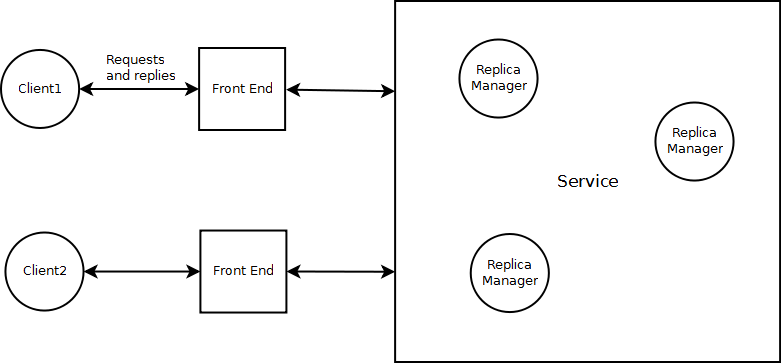
\includegraphics[width=0.7\textwidth]{img/replicationmodel}
	\end{center}
	\caption{Basic architectural model for the management of replicated data.}
	\label{fig:replicationmodel}
\end{figure}



Replica managers provide a service, i.e. access to objects, to the clients. Clients indirectly access object through the methods listed in \textbf{table 1}. The front end handles the client requests and uses messages to communicate with the replica managers. This abstraction layer ensures replication transparency at the client side [1].


\begin{table}
	\caption{Replica manager service API.}
	\label{tab:api:}
	\begin{tabular}{p{150px} | p{250px}}
		\textbf{Operation} & \textbf{Description} \\
		\hline
		readOnlyRequest (object) & \emph{Template method for an invocation by the client on an object with no updates on the object itself.} \\
		updateRequest (object) & \emph{Template method for an invocation by the client on an object, which alteres the state of the object.} \\
		\hline
	\end{tabular}
\end{table}

Coulouris et al. [1] list five phases in which the request is handles by the system:
\begin{enumerate}
	\item \textbf{Request} : The front end issues a request to one or more replica managers, either through unicast or through multicast. In the first case the replica manager will propagate the message to other replica managers.
	\item \textbf{Coordination} : Replica managers decide whether or not the request can be applied, i.e. the request will not introduce inconsistencies, and how the requests will be ordered. Possible ordering policies are for example FIFO, causal or total ordering.
	\item \textbf{Execution} : The request is executed by the replica managers.
	\item \textbf{Agreement} : The replica managers decide whether or not the commit the results of the request.
	\item \textbf{Response} : One or more replica managers communicate the result to the front end.
\end{enumerate}


\subsection{Group views}

The size of the set of replica managers may be be constant, i.e. membership is static, or vary, i.e. membership is dynamic. To manage this kind of groups, the group communication paradigm is often applied; particularly in the case of dynamic membership where the join and leave operations are concerned [1].

To manage groups, \emph{group views} are used. These are ordered lists of the current group members. Each group member has a unique process identifier. Group views are generated as members join or leave, after processes are notified of changes through view delivery. Correct view delivery requires a number of guarantees to be met [1]:
\begin{itemize}
	\item \textbf{Order} : If a processe delivers views v(g) and v'(g), then no other process will deliver v'(g) before v(g).
	\item \textbf{Integrity} : If a process delivers a view, then that process is part of the view.
	\item \textbf{Non-triviality} : A process q that is indefinitely reachable from a process p will always be in the views that p delivers.
\end{itemize}
In the case of \emph{view-synchronous group communication} additional constraints are to be met. \textbf{Figure 2} gives an overview of allowed and disallowed scenarios based on the following requirements [1]:
\begin{itemize}
	\item \textbf{Agreement} : Correct processes deliver the same sequence of views and set of messages within any given view.
	\item \textbf{Integrity} : If a correct process delivers a message m, this process will not deliver m again.
	\item \textbf{Validity} : Correct processes always deliver the messages that they send.
\end{itemize}



\begin{figure}
        \centering
        \begin{subfigure}[t]{0.4\textwidth}
                                        \centering
                                        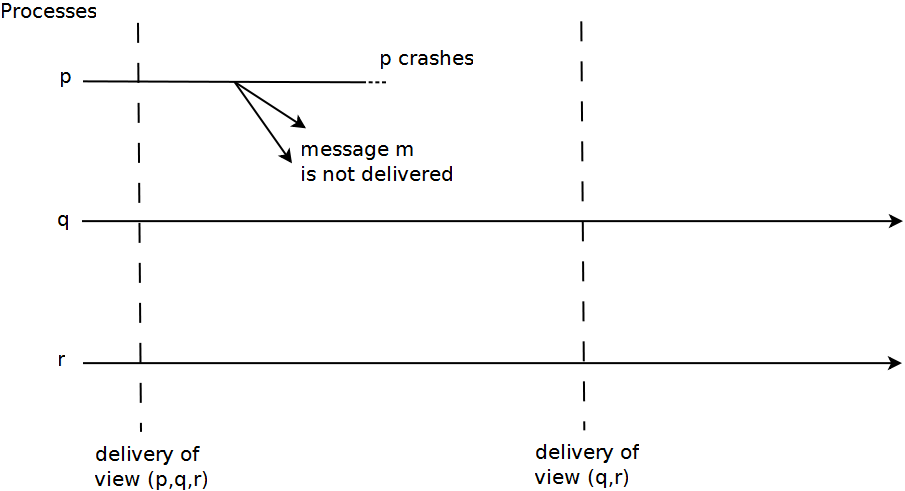
\includegraphics[width=\textwidth]{img/viewsynchronousgroupcommunication_a}
                                        \caption{Allowed case where the messages are not delivered and process p crashes.}
                                        \label{figure:viewsynchronousgroupcommunication:a}
        \end{subfigure}%
        ~
        \begin{subfigure}[t]{0.4\textwidth}
                                        \centering
                                        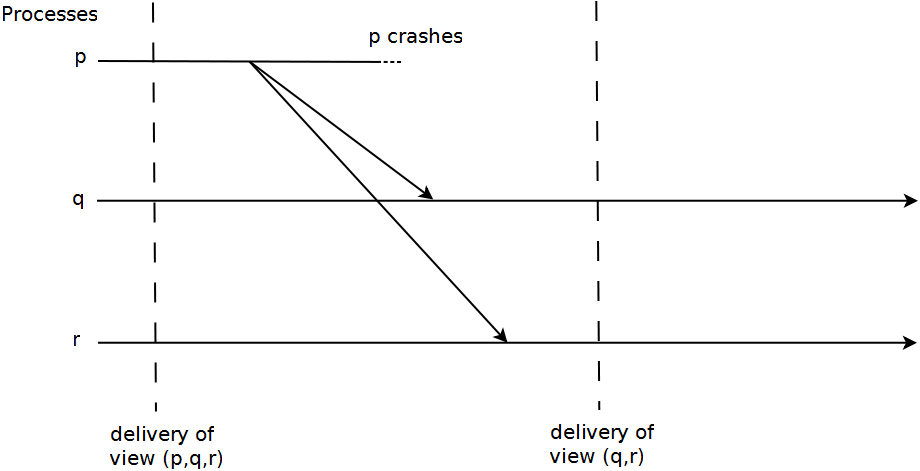
\includegraphics[width=\textwidth]{img/viewsynchronousgroupcommunication_b}
                                        \caption{Allowed case where the messages are delivered before the delivery of view (q,r).}
                                        \label{figure:viewsynchronousgroupcommunication:b}
        \end{subfigure}
        ~
        \begin{subfigure}[t]{0.4\textwidth}
                                        \centering
                                        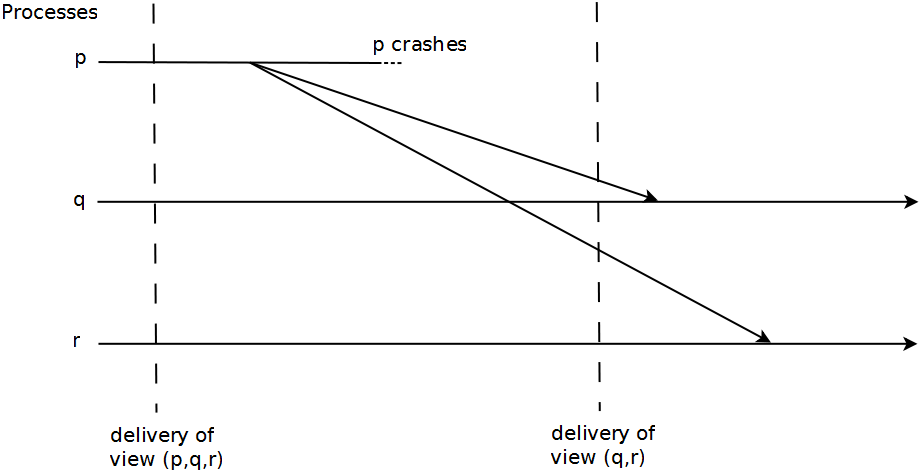
\includegraphics[width=\textwidth]{img/viewsynchronousgroupcommunication_c}
                                        \caption{Disallowed case where the messages are delivered after the delivery of view (q,r) which does not contain the crashed process p.}
                                        \label{figure:viewsynchronousgroupcommunication:c}
        \end{subfigure}
        ~
        \begin{subfigure}[t]{0.4\textwidth}
                                        \centering
                                        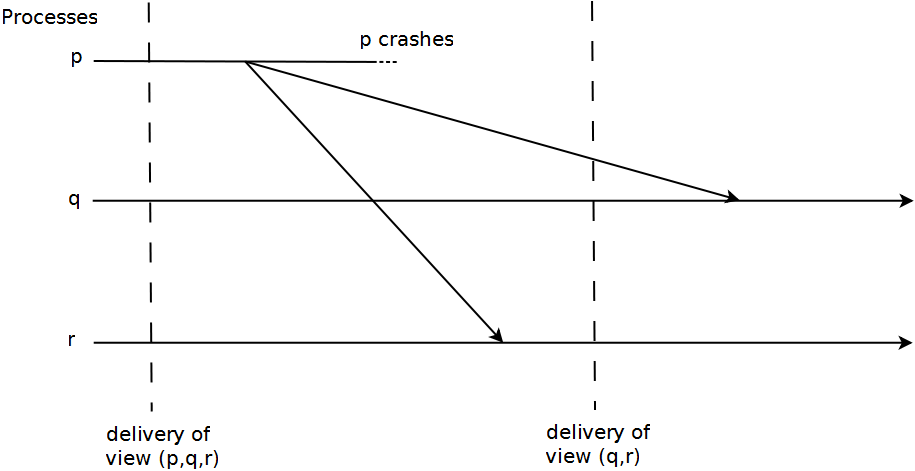
\includegraphics[width=\textwidth]{img/viewsynchronousgroupcommunication_d}
                                        \caption{Disallowed case where the messages are delivered in an incorrect order with regard to view delivery of (q,r).}
                                        \label{figure:viewsynchronousgroupcommunication:d}
        \end{subfigure}
        \caption{A selection of the screens used in the user study with paper prototype.}%
        \label{figure:viewsynchronousgroupcommunication}%
\end{figure}


View-synchronous group communication can be used to perform state transfer from the current group to new members. To ensure that the transferred state is not corrupt, the execution is usually temporary suspended. When the transfer is complete, the coordinator sends a message to the group members to continue.

The goal of group views is to increase fault-tolerance and transparency. As members crash or become unreachable, they are marked "suspicious" and may be excluded from the group by the membership service. This introduces a design challenge, as when excluding processes that are falsely excluded, resources and processing power may be (temporary) lost [1].

Another design decision has to be made in how to handle network partitions. Two general approaches exist: either the group is reduced, keeping only the primary-partition, or the group is partitionable into subgroups that can continue working independently [1].



\subsection{Fault tolerance}

The goal of fault tolerant systems is to "provide a service that is correct despite up to f process failures" [1]. This can be achieved by replicating data and functionality at replica managers. Correctness of replicated objects is subject to a number of criteria, which can vary in strictness.

\emph{Linearizability} is a strong correctness requirement. Consider a sequence of operation invocations and responses, called a \emph{history}, $o_{2,0}$, $o_{2,1}$, $o_{1,0}$, $o_{2,2}$, $o_{1,1}$, $o_{1,2}$, ..., where \emph{i} represents a client performing an operation \emph{j} for an operation $o_{i,j}$. \textbf{Figure 3 (a)} shows an overview of this setup. "A replicated shared object is linearizable if for any execution there is some interleaving of the series of operations issued by all clients that satisfies the following criteria" [1] :
\begin{itemize}
	\item The interleaved sequence of operations meets the specification of a (single) correct copy of the objects.
	\item The order of operations in the interleaving is consistent with the real times at which the operations occurred in the actual execution.
\end{itemize}
\textbf{Figure 3 (b)} shows how the operations in the history can be re-ordered. If there exists an ordering for which the previous conditions are met, the system is linearizable. In \textbf{figure 3 (c)} the new ordering did not meet the requirement.


\begin{figure}
        \centering
        \begin{subfigure}[t]{0.3\textwidth}
                                        \centering
                                        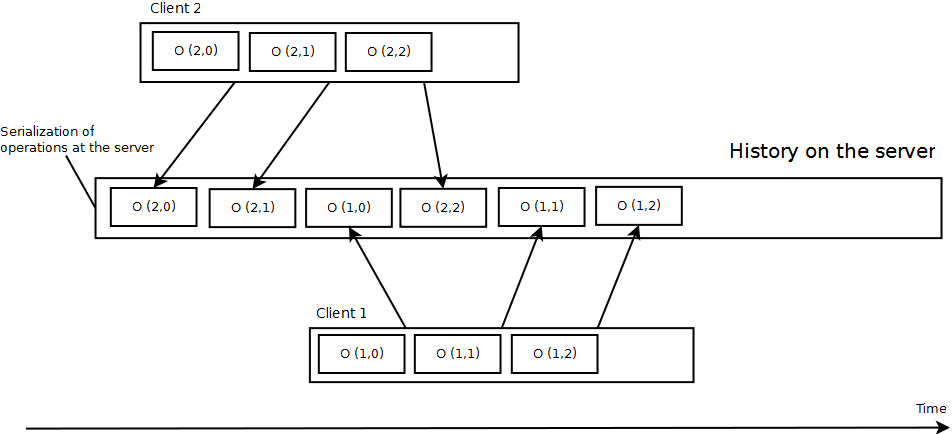
\includegraphics[width=\textwidth]{img/linearizability_1}
                                        \caption{Two clients executing operations on a replicated object managed by a server. The operations are serialized by the server into a certain sequence.}
                                        \label{figure:linearizability:a}
        \end{subfigure}%
        ~
        \begin{subfigure}[t]{0.3\textwidth}
                                        \centering
                                        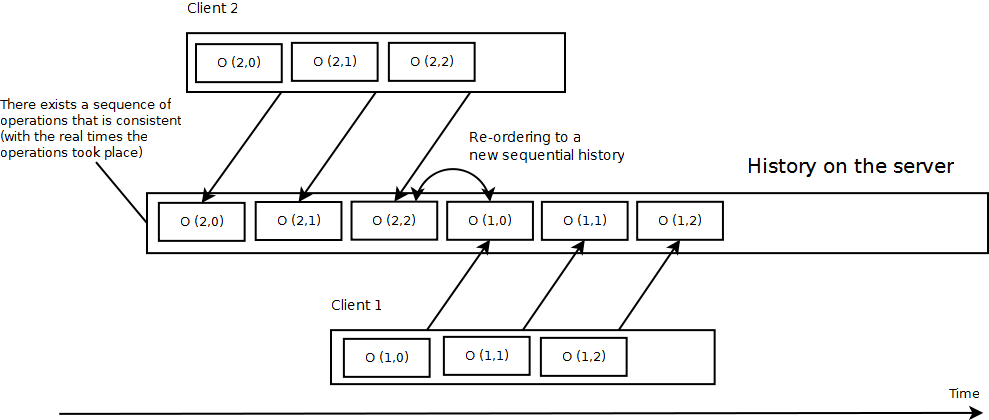
\includegraphics[width=\textwidth]{img/linearizability_2}
                                        \caption{The order of operations can be altered (serializibility) to obtain a new sequence that is consistent with the real times at which the operations occurred in the actual execution.}
                                        \label{figure:linearizability:b}
        \end{subfigure}
        ~
        \begin{subfigure}[t]{0.3\textwidth}
                                        \centering
                                        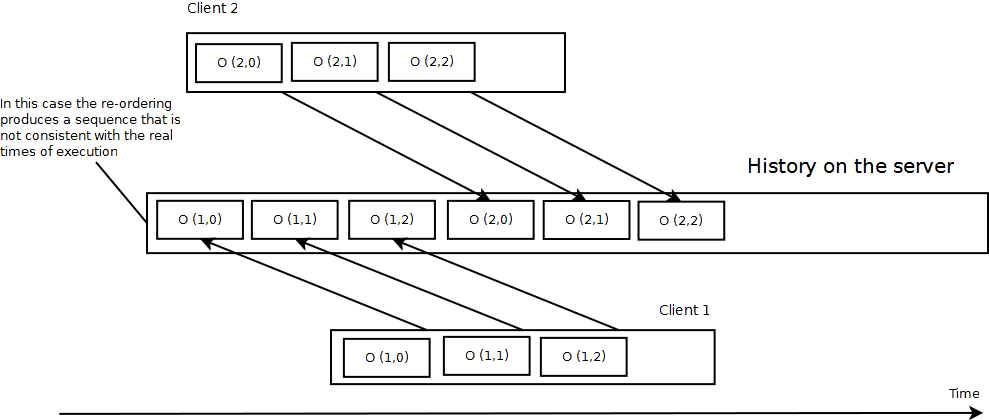
\includegraphics[width=\textwidth]{img/linearizability_3}
                                        \caption{The new sequence that is consistent not with the real times at which the operations occurred in the actual execution.}
                                        \label{figure:linearizability:c}
        \end{subfigure}
        \caption{}
        \label{figure:linearizability}
\end{figure}


\emph{Sequential consistency} is an example of a weak correctness critrium. The requirements for sequential consistency are the following:
\begin{itemize}
	\item The interleaved sequence of operations meets the specification of a (single) correct copy of the objects.
	\item The order of operations in the interleaving is consistent with the program order in which each individual client executed them.
\end{itemize}
As a result, the situation in \textbf{figure 3 (c)} is valid under a sequential consistency requirement. The absolute times are not important top obtain sequential consistency, just the order of events corresponding the clients seperately. It should be clear that sequential consistency is a much weaker constraint than linearizability. There may still be inconsistencies in the overal history, despite equential consistency. For example [2] when two clients try to lock an object, one lock will be successful and the other won't. In the case of sequential consistency, it is possible that the negative response is ordered before the successful response, which is not consistent with the sequential definition of the object, i.e. the first one to lock should have gotten a response of success.


\subsubsection{Passive replication}

The model for \emph{passive replication}, the so-called \emph{primary backup model of replication for fault tolerance}, consists out of primary replica manager and a collection of secondary replica managers or "backups". All operations are processed by the primary replica manager and afterwards changes are propagated to the backups. If the primary replica manager should fail, one of the backups is promoted to primary replica manager [1]. \textbf{Figure 4} shows an overview of this model.


\begin{figure}
	\begin{center}
		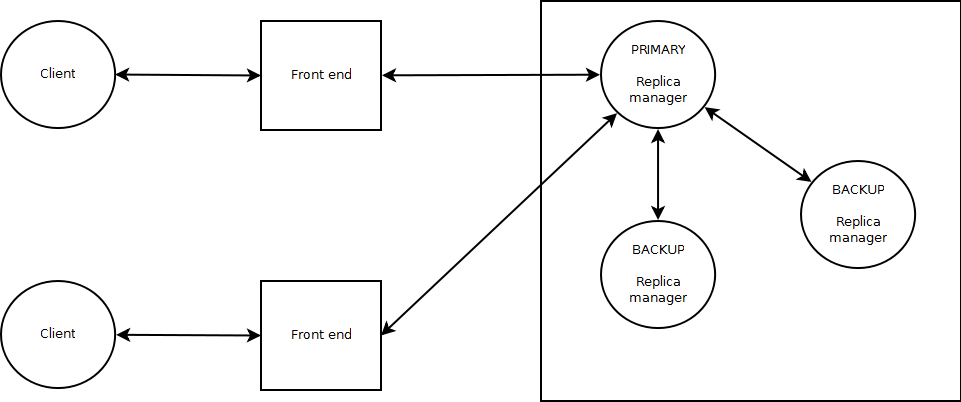
\includegraphics[width=0.7\textwidth]{img/passivereplication}
	\end{center}
	\caption{Passive replication model for fault tolerance.}
	\label{fig:passivereplication}
\end{figure}

The following steps occur when an operation is performed by a client [1]:
\begin{enumerate}
	\item \textbf{Request} : The front end issues the request, containing a unique identifier, to the primary replica manager.
	\item \textbf{Coordination} : The primary takes each request anatomically, in the order in which it receives it. It checks the unique identifier, in case it has already executed the request, and if so, it simply resends the response.
	\item \textbf{Execution} : The primary executes the request and stores the response.
	\item \textbf{Agreement} : If the request is an update, then the primary sends the updated state, the response and the unique identifier to all the backups. The backups send an acknowledgement.
	\item \textbf{Response} : The primary responds to the front end, which hands the response back to the client.
\end{enumerate}

The primary sequences all the operations upon the shared objects, so as long as the primary is correct, the system is linearizable. In the case that the primary fails, however, to ensure linearizability, the primary replica manager has to be replaced by a unique backup, and the remaining replica managers agree which operations had been performed when the replacement primary takes over. This will be the case if the replica managers apply view-synchronous group communication to send updates to the backups [1].



\subsubsection{Active replication}

In \emph{active replication} the replica managers are state machines with equivalent status and organized as a group. The front end multicasts requests to the group. Within the group each manager processes the requests independently in the same manner and reply individually to the front end [1]. \textbf{Figure 5} shows the model for active replication.

\begin{figure}
	\begin{center}
		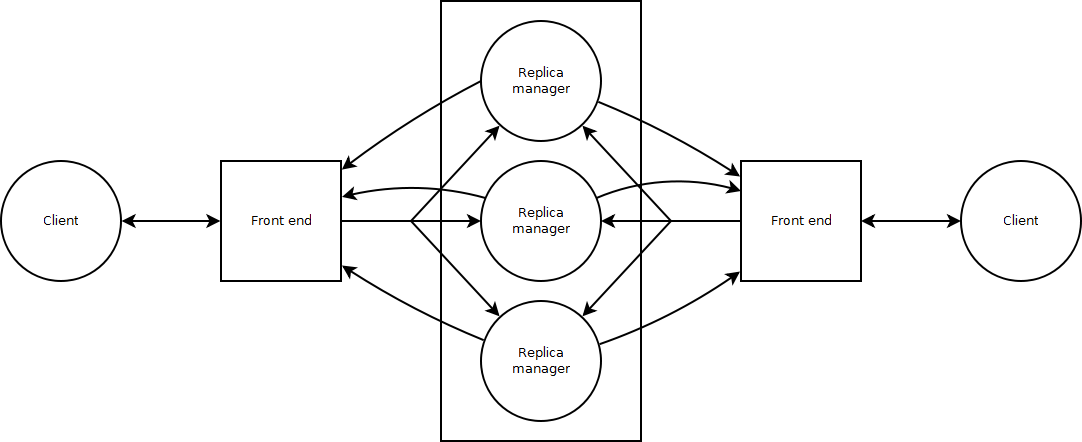
\includegraphics[width=0.7\textwidth]{img/activereplication}
	\end{center}
	\caption{Active replication model for fault tolerance.}
	\label{fig:activereplication}
\end{figure}


The following steps occur when an operation is performed by a client [1]:
\begin{enumerate}
	\item \textbf{Request} : The front end attaches a unique identifier to the request and multicasts it to the group of replica managers, using a totally ordered, reliable multicast primitive. The front end is assumed to fail by crashing at worst.It does not issues the next request until it has received a response.
	\item \textbf{Coordination} : The group communication system delivers the request to every correct replica manager in the same (total) order.
	\item \textbf{Execution} : Every replica manager executes the request. Since they are state machines and since requests are delivered in the same total order, correct replica managers all process the request identically. The response contains the client's unique request identifier.
	\item \textbf{Agreement} : No agreement phase is needed, because of multicast delivery semantics.
	\item \textbf{Response} : Each replica manager sends its response to the front end. The number of replies that the front end collects depends upon the failure assumptions and the multicast algorithm.
\end{enumerate}

The system is sequentially consistent, but does not achieve linearizability since the total ordering is not necessarily the same as the real-time order in which the clients made their requests [1].

Crashes of replica managers have little impact on the performance in active replication, as the remaining replica managers continue to work as usual. Because the front end can compare the replies it receives, the system is less prone to Bynzantine failures [1].


\subsubsection{Comparison: active and passive replication}


\begin{table}
	\caption{Comparison between passive and active replication.}
	\label{tab:compare:replication:faulttolerance}
	\begin{tabular}{p{80px} | p{155px} | p{155px}}
															& \textbf{Passive} & \textbf{Active} \\
		\hline
		\textbf{Correctness} 			& Support for linearizability. & Support up to sequential consistency. \\
		\textbf{Fault tolerance} 	& The system requires f+1 replica managers to survive up to f process crashes. & For f Byzantine failures, the system requires 2f+1 replica managers to ensure that the system continues to function correctly. This is because the front collects f+1 replies before passing on the results to the client. \\
		\textbf{Efficiency} 			& View-synchronous group communication is required to support linearizability, but introduces a significant overhead. In a variation where read requests are handled by backups to improve performance, the system looses its linearizability property, but maintains sequential consistency. & As managers work independently within te group, crashes have no impact on efficiency. The group communication is relatively cheap as no view-synchronous communication is required. \\
		\hline
	\end{tabular}
\end{table}




\section{Highly available services: examples of systems using replication}

\subsection{The Coda file system}


The Coda file system is based on the Andrew File System (AFS). It was developed to address additional requirements for file systems, in particular to provide high availability in presence of disconnected operations. Of course, Coda retains the original goals of AFS with regard to scalability and the emulation of UNIX file semantics. Coda tries to meet the following three additional requirements under the general heading of constant data availability [1,2]:

\begin{enumerate}
	\item \textbf{Performance} : In large-scale distributed systems this availability requirement becomes more important, as the limited form of replication offered by AFS on read-only volumes doesn't scale well for accessing widely shared files.
	\item \textbf{Fault tolerance} : The availability of AFS services was to be improved as failures (or scheduled interruptions) of servers and network components could make these services inaccessible for significant periods of time.
	\item \textbf{Disconnect operations due to mobility} : Finally, mobile computers disconnect and reconnect frequently leading to an availability requirement of files the user may need despite being disconnected [1].
\end{enumerate}

The design of Coda relies on the replication of file volumes to achieve a higher throughput of file access operations and a greater degree of fault tolerance. Coda also makes use of AFS's client caching extension [1]. Coda enhances availability both by [1]:
\begin{itemize}
	\item Replication of files across servers. The advantages of replicating file volumes on multiple servers are [1]:
		\begin{itemize}
			\item As long as at least one replica is accessible the client can access the files in that replicated volume.
			\item System performance can be improved by sharing some of the load, i.e. client requests on replicated volumes, between the servers holding replicas.
		\end{itemize}
	
	\item The ability of clients to operate entirely out of their caches. Coda will try to predict which files will be needed by a user and cache them in case of disconnection with the network.
\end{itemize}



\subsubsection{The Coda architecture}

\paragraph{Vice (server) and Venus (client) processes}

\textbf{Figure 6} shows an overview of the Coda file system architecture. Similar to AFS, Coda runs \emph{Venus} processes at the client computers and \emph{Vice} processes at file server computers. The Vices are the replica managers, and the Venuses are a hybrid of front ends and replica managers. A Venus plays the front end's role of hiding the service implementation from local client processes, but since they manage a local cache of files they are also replica managers.

\begin{figure}
	\begin{center}
		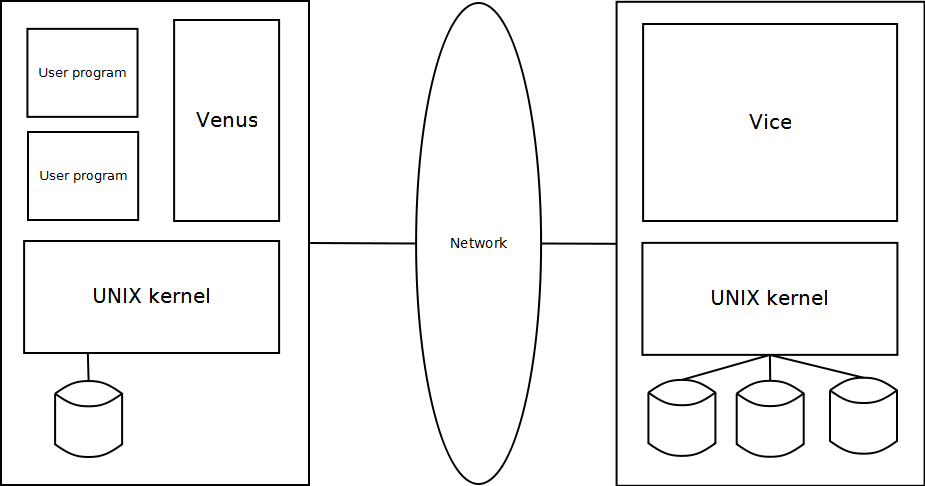
\includegraphics[width=0.7\textwidth]{img/afs}
	\end{center}
	\caption{Coda file system architecture (AFS-based).}
	\label{fig:coda}
\end{figure}



\paragraph{The volume storage group (VSG)}

A volume storage group (VSG) is the set of servers that holds replicas of a file volume. As servers become inaccessible as a result of network or server failures, the client can usually only access a subset of the VSG, known as the available volume storage group (AVSG). A disconnected operation occurs when the AVSG is empty [1].



\subsubsection{Replication and consistency}

The Coda servers are the focal point to provide quality of service, as cached file copies residing on client computers are regarded as less reliable than those at the servers. These files are periodically revalidated against the version at the servers. In presence of network partitions updated files may cause conflicts with other replicas when the network is restored [1].

Coda uses an optimistic replication strategy, i.e. files can be modified in presence of network partitions or during disconnected operations.


\paragraph{Coda version vector}

Each version of a file has a \emph{Coda version vector} (CVV) containing a timestamp with one element for each server in the corresponding VSG [1]. When a modified file is closed, the Venus process sends an update message with the current CVV and the new contents for the file to the AVSG. If the CVV is greater than the one currently held at the AVSG, the new contents for the file are stored and a positive acknowledgement is returned. The Venus process then computes a new CVV with modification counts increased for the servers that responded positively to the update message and distributes the new CVV to the members of the AVSG. Note that AVSG is only a subset of the VSG, so possibly not all members will receive the new CVV [1].

The CVV can be used for resolving file conflicts as follows. For timestamps of two CVVs $v_{1}$ and $v_{2}$, there are two general cases [1]:
\begin{itemize}
	\item If the CVV at one of the sites is greater than or equal to all the corresponding CVVs at the other sites then there is no conflict.
	\item When neither $v_{1} \leq v_{2}$ nor $v{1} \geq v_{2}$ holds for two CVVs then there is a conflict: each replica reflects at least one update that the other does not reflect. Coda does not, in general, resolve conflicts automatically. The file is marked as \emph{inoperable} and the owner of the file is informed of the conflict.
\end{itemize}



\paragraph{Accessing replicas and update semantics}

AFS's original \emph{callback promise} mechanism, is extended and depends on an additional mechanism for the distribution of updates to each replica. The strategy used on open and close on the replicas is a variant of the \emph{read-one/write-all} approach [1]. \textbf{Table 3} lists the open and close operation specifics.


\begin{table}
	\caption{File open and close operation in Coda.}
	\label{tab:api:coda}
	\begin{tabular}{p{150px} | p{250px}}
		\textbf{Operation} & \textbf{Description} \\
		\hline
		open 	& This operation consists of the following steps. If a copy of the file is not present in the local cache:
				\begin{enumerate}
					\item The client choses a preferred server from the AVSG for the file.
					\item The client requests a copy of the file attributes and contents from the preferred server.
					\item The client checks with all the other members of the AVSG to verify that the copy is the latest available version. If not, a member of the AVSG with the latest version is made the preferred site, the file contents are refetched and the members of the AVSG are notified that some members have stale replicas.
					\item When the fetch has been completed, a callback promise is established at the preferred server.
				\end{enumerate} \\
		close & On close, copies of modified files are broadcast in parallel to all of the servers in the AVSG using \emph{multicast remote procedure calling protocol}. This has two notable effects:
				\begin{enumerate}
					\item It maximizes the \textit{probability} that every replication site for a file has the current version at all times. It doesn't guarantee it, because the AVSG does not necessarily include all the members of the VSG.
					\item It minimizes the server load by giving clients the responsibility for propagating changes to the replication sites in the normal case.
				\end{enumerate} \\
		\hline
	\end{tabular}
\end{table}



The update semantics for Coda are a little different to those in AFS. The single server \textit{S} referred to in the currency guarantees for AFS is replaced by a set of servers \textit{S}, i.e. the VSG for a file \textit{F} and the client \textit{C} can access a subset of servers \textit{s}, i.e., the AVSG for that file seen by \textit{C}. \textit{T} is again the maximum time that for which a client can remain unaware of an update elsewhere to the cached file [1]. In addition the following predicates are used:
\begin{itemize}
	\item $latest(F, s, T)$ : The current value of \textit{F} at \textit{C} was the latest across all the servers in s at some instant in the last \textit{T} seconds and that there were no conflicts among the copies of \textit{F} at that instant;
	\item $lostCallback(s, T)$ : A callback was sent by some member of \textit{s} in the last \textit{T} seconds and was not received at \textit{C};
	\item $conflict(F,s)$ : The values of \textit{F} at some servers in \textit{s} are currently in conflict.
\end{itemize}


The currency guarantees are then summarized as follows [1]. In each definition except the last there are two cases [1]:
\begin{enumerate}
	\item $s \neq \emptyset$ : The AVSG is not empty, i.e., the client is not disconnected.
	\item $s = \emptyset$ : The disconnected operation.
\end{enumerate}

\textbf{After succesfull open} : The guarantee offered by a successful open is that either that the most recent copy of \textit{F} is provided from the current AVSG, or a locally cached copy of \textit{F} is used if one is available, if no server is accessible:

$(s \neq \emptyset \wedge (latest(F, s, 0) \vee (latest(F, s, T) \wedge lostCallback(s, T) \vee inCache(F))))$ \\
$\vee$ \\
$(s = \emptyset \wedge inCache(F))$ \\

\textbf{After failed open :}

$(s \neq \emptyset \wedge conflict(F, s)) \vee (s = \emptyset \wedge \neg inCache(F))$ \\

\textbf{After succesfull close} : A successful close guarantees that the file has been propagated to the currently accessible set of servers, or, if no server is available, that the file has been marked for propagation at the earliest opportunity.

$(s \neq \emptyset \wedge updated(F, s)) \vee (s = \emptyset)$ \\

\textbf{After failed close :}

$(s \neq \emptyset \wedge conflict(F, s))$ \\








\subsubsection{Caching}


\paragraph{Cache coherence}

The Coda currency guarantees stated earlier mean that the Venus process at each client must detect the following events within \textit{T} seconds of their occurrence [1]:
\begin{itemize}
	\item \textbf{AVSG size changes} : Enlargement of an AVSG (due to the accessibility of a previously inaccessible server), or shrinking of an AVSG (due to a server becoming inaccessible);
	\item \textbf{Callback event loss} : Since maintaining callback state in all the members of an AVSG would be expensive, the callback promise is maintained only at the preferred server. However, the preferred server for one client need not be in the AVSG of another client. If this is the case, an update by the second client will not cause a callback to the first client.
\end{itemize}


\subparagraph{AVSG size changes}

Venus (client) sends a probe message to all the servers in VSGs of the files that it has in its cache every \textit{T} seconds. Responses will be received only from accessible servers. The following cases can be distinguished with regard to callback reponses:
\begin{itemize}
	\item \textbf{Venus receives a response from a server that was previously inaccessible} : Venus enlarges the corresponding AVSG. As the cached copy may no longer be the latest version available, Venus will also drop the callback promises on any files that it holds from the relevant volume.
	\item \textbf{Venus fails to receive a response from a previously accessible server} : Venus shrinks the corresponding AVSG. Unless the preferred server is lost, no callback changes are required.
	\item \textbf{The preferred server is lost} : All callback promises from that server must be dropped.
	\item \textbf{A response indicates that a callback message was sent but not received} : The callback promise on the corresponding file is dropped.
\end{itemize}


\subparagraph{Disjunct AVSGs}

Venus is sent a \emph{volume version vector} (volume CVV) in response to each probe message, containing a summary of the CVVs for all of the files in the volume. If Venus detects any mismatch between the volume CVVs, then some members of the AVSG must have some file versions that are not up-to-date. Although the outdated files may not be the ones that are in its local cache, Venus makes a pessimistic assumption and drops the callback promises on all of the files that it holds from the relevant volume [1].


\paragraph{Cache miss and disconnected operation}

In disconnected operation (when none of the servers for a volume can be accessed by the client) a cache miss prevents further progress and the computation is suspended until the connection is resumed or the user aborts the process. It is therefore important to load the cache before disconnected operation commences so that cache misses can be avoided [1].

\subparagraph{Selecting files to retain in the cache}

If a client is disconnected for an extended period of time, it is likely that files or directories will be referenced that are not in the cache. To alleviate this problem Coda allows users to specify a prioritized list of files and directories that Venus should strive to retain in the cache. Objects at the highest level are identified as \emph{sticky} and these must be retained in the cache at all times. If the local disk is large enough to accommodate all of them, the user is assured that they will remain accessible [1].

\subparagraph{Reintegration after disconnect operation}

When disconnected operation ends, a process of reintegration begins. For each cached file or directory that has been modified, created or deleted during disconnected operation, Venus executes a sequence of update operations to make the AVSG replicas identical to the cached copy. Reintegration proceeds top-down from the root of each cached volume [1].




\subsection{Gossip framework}

The goal of the Gossip framework is implementing highly available services by replicate data close to points where groups of clients need it [3]. Gossip is not fault tolerant. A framework implies that it is configurable with multiple degrees of freedom. The consequence of this is that it can be used for a variety of applications [3].

\begin{figure}
	\begin{center}
		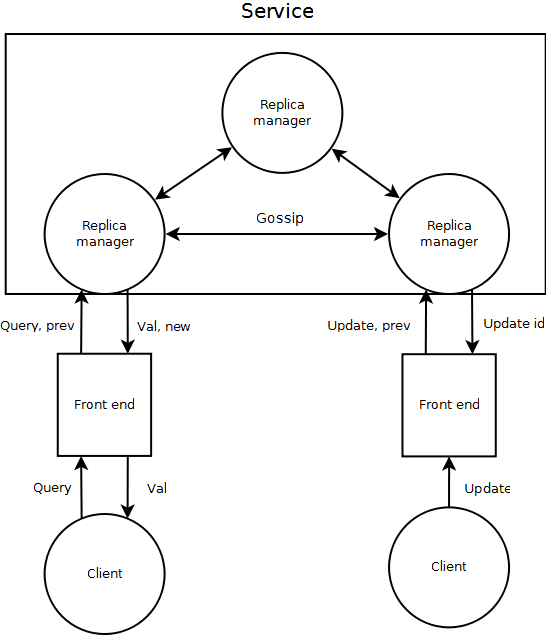
\includegraphics[width=0.6\textwidth]{img/gossiparchitecture}
	\end{center}
	\caption{The Gossip framework architecture.}
	\label{fig:gossiparchitecture}
\end{figure}


The front end sends operations to any RM that is available and has a reasonable response time. There are two types of operations [3]:
\begin{itemize}
	\item \textbf{Queries} : Read-only operations;
	\item \textbf{Updates} : Change state
\end{itemize}


\subsection{Bayou}

The goals of the Bayou model are data replication for high availability, but with weaker guarantees than sequential consistency, and coping with variable connectivity [3].




\section*{References}

\begin{enumerate}[1]
	\item G. Coulouris, J. Dollimore, T. Kindberg and G. Blair, "Distributed Systems: Concepts and Design (5th Edition)", M. Horton, Red., Addison-Wesley, 2011, p. 1063.
	\item Wikipedia, 2013, "Linearizability | Wikipedia", online, available at:  http://en.wikipedia.org/wiki/Linearizability
	\item W. Joosen, 2013, "Distributed Systems: Replicated Data - Part 1",  iMinds-DistriNet KULeuven
\end{enumerate}

